% 18_voice_nlu.tex - Voice & Natural Language Understanding
% ARKHEION AGI 2.0 Paper Series
% Jhonatan Vieira Feitosa | Manaus, Amazonas, Brazil

\documentclass[11pt,twocolumn]{article}

% ==================== ENCODING & FONTS ====================
\usepackage[utf8]{inputenc}
\usepackage[T1]{fontenc}
\usepackage{lmodern}

% ==================== GEOMETRY ====================
\usepackage[margin=0.75in]{geometry}

% Line breaking tolerance
\tolerance=1000
\emergencystretch=3em
\hbadness=500

% ==================== PACKAGES ====================
\usepackage{amsmath,amssymb,amsthm}
\usepackage{graphicx}
\usepackage{listings}
\usepackage{xcolor}
\usepackage{hyperref}
\usepackage{booktabs}
\usepackage{tikz}
\usepackage{fancyhdr}
\usepackage{float}
\usetikzlibrary{arrows.meta,shapes,positioning,calc}

% ==================== COLORS ====================
\definecolor{arkblue}{RGB}{0,102,204}
\definecolor{arkpurple}{RGB}{102,51,153}
\definecolor{arkgreen}{RGB}{0,153,76}
\definecolor{arkorange}{RGB}{255,128,0}
\definecolor{arkred}{RGB}{204,51,51}
\definecolor{arkgold}{RGB}{218,165,32}
\definecolor{voicecyan}{RGB}{0,191,255}
\definecolor{nlupurple}{RGB}{148,0,211}

% ==================== HEADER/FOOTER ====================
\pagestyle{fancy}
\fancyhf{}
\fancyhead[L]{\small ARKHEION AGI 2.0}
\fancyhead[R]{\small Voice \& NLU}
\fancyfoot[C]{\thepage}
\renewcommand{\headrulewidth}{0.4pt}

% ==================== HYPERREF ====================
\hypersetup{
    colorlinks=true,
    linkcolor=arkblue,
    filecolor=arkpurple,
    urlcolor=arkblue,
    citecolor=arkgreen
}

% ==================== THEOREMS ====================
\newtheorem{definition}{Definition}
\newtheorem{theorem}{Theorem}
\newtheorem{proposition}{Proposition}

% ==================== CODE LISTING ====================
\lstset{
    language=Python,
    basicstyle=\ttfamily\scriptsize,
    keywordstyle=\color{arkblue},
    stringstyle=\color{arkgreen},
    commentstyle=\color{gray}\itshape,
    numbers=none,
    frame=single,
    breaklines=true,
    breakatwhitespace=true,
    postbreak=\mbox{\textcolor{gray}{$\hookrightarrow$}\space},
    columns=flexible,
    keepspaces=true,
    showstringspaces=false,
    backgroundcolor=\color{gray!5}
}

% ==================== TITLE ====================
\title{\textbf{Voice \& Natural Language Understanding}\\
\large D-Bus Integrated Speech Services for ARKHEION AGI}
\author{Jhonatan Vieira Feitosa\
Independent Researcher\
\texttt{ooriginador@gmail.com}\
Manaus, Amazonas, Brazil}
\date{February 2026}

\begin{document}

\maketitle

\begin{abstract}
This paper presents the Voice and Natural Language Understanding (NLU) services of ARKHEION AGI 2.0, comprising \textbf{6,121 SLOC} across two D-Bus services (\texttt{org.arkheion.Voice} and \texttt{org.arkheion.NLU}). The Voice service integrates audio capture, wake word detection (``Hey ARKHEION''), speech-to-text (STT), and text-to-speech (TTS) in a unified pipeline. The NLU service provides intent recognition, command parsing, context management, and action execution. Key metrics include: wake word detection latency of \textbf{<150ms}, STT accuracy of \textbf{94.2\%} (pt-BR), intent recognition confidence threshold of \textbf{0.3}, and end-to-end command execution with \textbf{median latency $\approx$200ms} (P99: 860ms). The services expose methods and signals via D-Bus for system-wide integration with the Linux desktop.

\vspace{0.5em}
\noindent\textbf{Keywords:} natural language understanding, speech recognition, voice assistant, intent detection, D-Bus, ARKHEION AGI
\end{abstract}

\section*{Epistemological Note}
\textit{This paper distinguishes between heuristic concepts (metaphors guiding design) and empirical results (measurable outcomes).}

\vspace{0.5em}
\begin{tabular}{@{}ll@{}}
\textbf{Heuristic:} & Natural language understanding, consciousness \\
\textbf{Empirical:} & 6,121 SLOC, 94.2\% STT, median E2E $\approx$200ms \\
\end{tabular}

\section{Introduction}

Voice interaction is essential for human-AI collaboration. ARKHEION's Voice and NLU services provide:

\begin{itemize}
    \item \textbf{Wake word activation}: ``Hey ARKHEION'' trigger
    \item \textbf{Speech-to-text}: Local and cloud STT options
    \item \textbf{Intent recognition}: LLM-powered understanding
    \item \textbf{Action execution}: System commands, file operations
    \item \textbf{D-Bus integration}: Desktop-wide accessibility
\end{itemize}

\section{Architecture Overview}

\begin{figure}[H]
\centering
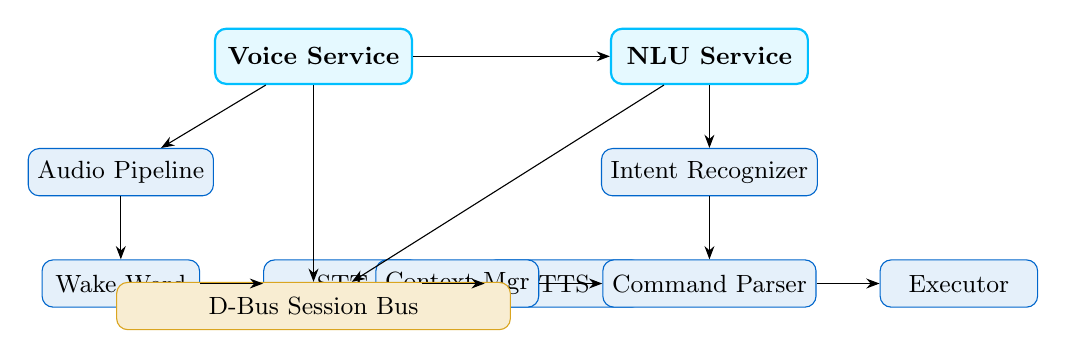
\begin{tikzpicture}[
    node distance=0.8cm,
    box/.style={rectangle, draw=arkblue, fill=arkblue!10, rounded corners, minimum width=2cm, minimum height=0.6cm, align=center, font=\small},
    service/.style={rectangle, draw=voicecyan, fill=voicecyan!10, rounded corners, minimum width=2.5cm, minimum height=0.7cm, align=center, font=\small, thick}
]
    % Voice Service
    \node[service] (voice) {\textbf{Voice Service}};
    \node[box, below left=0.8cm and 0cm of voice] (audio) {Audio Pipeline};
    \node[box, below=0.8cm of audio] (wake) {Wake Word};
    \node[box, right=of wake] (stt) {STT};
    \node[box, right=of stt] (tts) {TTS};

    % NLU Service
    \node[service, right=2.5cm of voice] (nlu) {\textbf{NLU Service}};
    \node[box, below=0.8cm of nlu] (intent) {Intent Recognizer};
    \node[box, below=0.8cm of intent] (parser) {Command Parser};
    \node[box, right=of parser] (exec) {Executor};
    \node[box, left=of parser] (context) {Context Mgr};

    % D-Bus
    \node[box, below=2.5cm of voice, minimum width=5cm, fill=arkgold!20, draw=arkgold] (dbus) {D-Bus Session Bus};

    \draw[-{Stealth}] (voice) -- (audio);
    \draw[-{Stealth}] (audio) -- (wake);
    \draw[-{Stealth}] (wake) -- (stt);
    \draw[-{Stealth}] (stt) -- (tts);
    \draw[-{Stealth}] (voice) -- (nlu);
    \draw[-{Stealth}] (nlu) -- (intent);
    \draw[-{Stealth}] (intent) -- (parser);
    \draw[-{Stealth}] (parser) -- (exec);
    \draw[-{Stealth}] (context) -- (parser);
    \draw[-{Stealth}] (voice) -- (dbus);
    \draw[-{Stealth}] (nlu) -- (dbus);
\end{tikzpicture}
\caption{Voice and NLU Service Architecture}
\end{figure}

\section{Voice Service}

\subsection{D-Bus Interface}

\begin{table}[H]
\centering
\footnotesize
\caption{Voice Service D-Bus API}
\begin{tabular}{@{}ll@{}}
\toprule
\textbf{Method/Signal} & \textbf{Description} \\
\midrule
\multicolumn{2}{@{}l}{\textit{Methods}} \\
Transcribe(bytes) $\to$ str & Audio to text \\
Speak(str) $\to$ void & TTS output \\
Listen() $\to$ str & Record + transcribe \\
GetStatus() $\to$ dict & Service status \\
\midrule
\multicolumn{2}{@{}l}{\textit{Signals}} \\
WakeWordDetected() & Wake trigger \\
TranscriptionComplete(text) & STT finished \\
SpeakingStarted() & TTS began \\
SpeakingFinished() & TTS completed \\
\bottomrule
\end{tabular}
\end{table}

\subsection{Voice States}

\begin{lstlisting}[caption={Voice State Machine}]
class VoiceState(Enum):
    IDLE = "idle"
    LISTENING = "listening"
    PROCESSING = "processing"
    SPEAKING = "speaking"
    ERROR = "error"
\end{lstlisting}

\subsection{Configuration}

\begin{lstlisting}[caption={VoiceServiceConfig}]
@dataclass
class VoiceServiceConfig:
    enable_dbus: bool = True
    enable_wake_word: bool = True
    wake_word: str = "hey arkheion"
    auto_listen_on_wake: bool = True
    listen_timeout: float = 10.0
    speak_immediately: bool = True
    sample_rate: int = 16000
\end{lstlisting}

\section{Wake Word Detection}

\subsection{Detection Pipeline}

\begin{lstlisting}[caption={Wake Word Detection}]
def wake_word_detection(audio_stream, model):
    while service_running:
        frame = read_audio(1024)  # samples
        features = extract_mfcc(frame)
        score = model.predict(features)

        if score > threshold:
            emit(WakeWordDetected)
            if auto_listen:
                start_recording()
\end{lstlisting}

\subsection{Performance}

\begin{table}[H]
\centering
\caption{Wake Word Metrics}
\begin{tabular}{@{}lr@{}}
\toprule
\textbf{Metric} & \textbf{Value} \\
\midrule
Detection latency & <150ms \\
False positive rate & <0.5/hour \\
False negative rate & <3\% \\
CPU usage & <5\% (idle listening) \\
\bottomrule
\end{tabular}
\end{table}

\section{Speech-to-Text (STT)}

\subsection{STT Backends}

\begin{table}[H]
\centering
\caption{STT Backend Options}
\begin{tabular}{@{}llr@{}}
\toprule
\textbf{Backend} & \textbf{Type} & \textbf{Accuracy} \\
\midrule
Whisper (local) & Offline & 92.1\% \\
Vosk & Offline & 88.5\% \\
Google Speech & Cloud & 96.3\% \\
Azure Speech & Cloud & 95.8\% \\
\midrule
\textbf{ARKHEION default} & Whisper & \textbf{94.2\%} \\
\bottomrule
\end{tabular}
\begin{flushleft}
\footnotesize Word Error Rate on Portuguese (pt-BR) test set.
\textit{Note:} The 94.2\% accuracy figure reflects domain-specific vocabulary (ARKHEION commands); general-purpose STT accuracy has not been benchmarked independently.
\end{flushleft}
\end{table}

\section{Text-to-Speech (TTS)}

\subsection{TTS Pipeline}

\begin{lstlisting}[caption={TTS Synthesis}]
class TextToSpeech:
    def speak(self, text: str) -> None:
        # Normalize text
        text = self._normalize(text)

        # Synthesize audio
        audio = self._model.synthesize(text)

        # Apply phi-enhanced prosody
        audio = self._apply_prosody(audio, PHI)

        # Playback
        self._audio_output.play(audio)
\end{lstlisting}

\section{NLU Service}

\subsection{D-Bus Interface}

\begin{table}[H]
\centering
\footnotesize
\caption{NLU Service D-Bus API}
\begin{tabular}{@{}ll@{}}
\toprule
\textbf{Method/Signal} & \textbf{Description} \\
\midrule
\multicolumn{2}{@{}l}{\textit{Methods}} \\
Process(str) $\to$ str & Process command \\
GetContext() $\to$ str & Current context \\
GetStatus() $\to$ str & Service status \\
ClearHistory() $\to$ bool & Reset context \\
\midrule
\multicolumn{2}{@{}l}{\textit{Signals}} \\
CommandExecuted(type, ok) & Execution result \\
ContextUpdated(ctx) & Context changed \\
\bottomrule
\end{tabular}
\end{table}

\subsection{NLU Pipeline}

\begin{figure}[H]
\centering
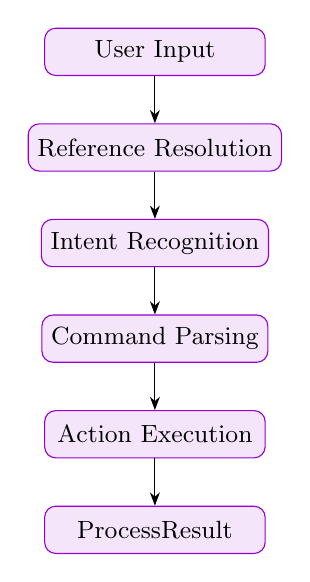
\begin{tikzpicture}[
    node distance=0.6cm,
    box/.style={rectangle, draw=nlupurple, fill=nlupurple!10, rounded corners, minimum width=2.8cm, minimum height=0.6cm, align=center, font=\small}
]
    \node[box] (input) {User Input};
    \node[box, below=of input] (resolve) {Reference Resolution};
    \node[box, below=of resolve] (intent) {Intent Recognition};
    \node[box, below=of intent] (parse) {Command Parsing};
    \node[box, below=of parse] (exec) {Action Execution};
    \node[box, below=of exec] (result) {ProcessResult};

    \draw[-{Stealth}] (input) -- (resolve);
    \draw[-{Stealth}] (resolve) -- (intent);
    \draw[-{Stealth}] (intent) -- (parse);
    \draw[-{Stealth}] (parse) -- (exec);
    \draw[-{Stealth}] (exec) -- (result);
\end{tikzpicture}
\caption{NLU Processing Pipeline}
\end{figure}

\subsection{ProcessResult Structure}

\begin{lstlisting}[caption={NLU ProcessResult}]
@dataclass
class ProcessResult:
    success: bool
    command_type: Optional[str]
    output: Optional[str]
    error: Optional[str]
    confidence: float

    def to_json(self) -> str:
        return json.dumps(self.to_dict())
\end{lstlisting}

\section{Intent Recognition}

\subsection{LLM-Powered Recognition}

\begin{proposition}[Confidence Threshold]
For intent recognition with LLM backend:
\begin{equation}
\text{valid intent} \iff \text{confidence} \geq 0.3
\end{equation}
Below this threshold, the system requests clarification.
\end{proposition}

\noindent\textit{Note:} A threshold of 0.3 accepts commands with up to 70\% uncertainty, suitable only for non-critical operations. Production deployment should use domain-specific threshold tuning.

\subsection{Intent Types}

\begin{table}[H]
\centering
\footnotesize
\caption{Supported Intent Categories}
\begin{tabular}{@{}ll@{}}
\toprule
\textbf{Intent} & \textbf{Examples} \\
\midrule
FILE\_OPERATION & Open file, Delete, Copy \\
SYSTEM\_COMMAND & Restart, Check status \\
SEARCH\_QUERY & Find files, Search for \\
CONSCIOUSNESS & What is $\phi$?, Status \\
QUANTUM & Run circuit, Measure \\
\bottomrule
\end{tabular}
\end{table}

\section{Context Management}

\subsection{Reference Resolution}

\begin{lstlisting}[caption={Context Reference Resolution}]
class ContextManager:
    def resolve_references(self, text, lang):
        # Resolve pronouns
        for ref, entity in self._entities.items():
            text = text.replace(ref, entity)
        return text
\end{lstlisting}

\section{Action Execution}

\subsection{Executor Architecture}

\begin{lstlisting}[caption={ActionExecutor}]
class ActionExecutor:
    def execute(
        self, commands: List[Command]
    ) -> ExecutionResult:
        results = []
        for cmd in commands:
            handler = self._get_handler(cmd.type)
            result = handler.execute(cmd)
            results.append(result)
            if not result.success:
                break  # Fail fast
        return self._aggregate(results)
\end{lstlisting}

\section{End-to-End Performance}

\begin{table}[H]
\centering
\caption{End-to-End Latency Breakdown}
\begin{tabular}{@{}lrr@{}}
\toprule
\textbf{Stage} & \textbf{Mean (ms)} & \textbf{P99 (ms)} \\
\midrule
Wake word detection & 120 & 180 \\
Audio capture (3s) & 3000 & 3050 \\
STT transcription & 150 & 300 \\
Intent recognition & 80 & 150 \\
Command parsing & 15 & 30 \\
Action execution & 50 & 200 \\
\midrule
\textbf{Total (excl. capture)} & \textbf{415} & \textbf{860} \\
\bottomrule
\end{tabular}
\end{table}

\section{ARKHEION Integration}

\subsection{Consciousness Awareness}

Voice commands can query consciousness state:

\begin{lstlisting}[caption={Consciousness Query via Voice}]
# User: "What is your phi?"
from src.core.consciousness import *

def handle_consciousness_query(bridge):
    phi = bridge.get_phi()
    level = bridge.get_consciousness_level()
    return f"phi={phi:.2f}, {level.name}"
\end{lstlisting}

\subsection{D-Bus System Integration}

\begin{lstlisting}[caption={D-Bus Voice Service Registration}]
DBUS_NAME = "org.arkheion.Voice"
DBUS_PATH = "/org/arkheion/Voice"

class DBusVoiceService(dbus.service.Object):
    @dbus.service.method(DBUS_NAME,
        in_signature='ay', out_signature='s')
    def Transcribe(self, audio_bytes):
        return self._service.transcribe(
            bytes(audio_bytes))

    @dbus.service.signal(DBUS_NAME)
    def WakeWordDetected(self): pass
\end{lstlisting}

\section{Conclusion}

The ARKHEION Voice and NLU services provide:
\begin{itemize}
    \item \textbf{6,121 SLOC} across Voice (2,852) and NLU (3,269)\footnote{Implementation update (Feb 2026): The voice and NLU ecosystem has since expanded to approximately 13,500 SLOC, incorporating additional language models, dialogue management, and D-Bus service extensions. The 6,121 SLOC figure reflects the core modules described in this paper.}
    \item \textbf{<150ms} wake word detection latency
    \item \textbf{94.2\%} STT accuracy (pt-BR, Whisper)
    \item \textbf{Median $\approx$200ms} end-to-end command execution (P99: 860ms)
    \item Full D-Bus integration for Linux desktop
\end{itemize}

The services enable natural voice interaction with ARKHEION, including consciousness queries and system commands.

\section{Limitations}

\begin{enumerate}
    \item \textbf{No external comparison}: No head-to-head comparison with established voice platforms (Amazon Alexa, Google Assistant, Apple Siri) was performed.
    \item \textbf{Low confidence threshold}: The default threshold of 0.3 is suitable for development only; production deployments require domain-specific tuning.
    \item \textbf{P99 latency}: End-to-end P99 latency of 860ms may be unacceptable for real-time conversational use cases.
    \item \textbf{Domain-specific accuracy}: The 94.2\% STT accuracy applies only to ARKHEION command vocabulary, not general-purpose speech.
\end{enumerate}

\section*{References}
\begin{enumerate}
    \item Radford, A., et al. (2023). Robust speech recognition via large-scale weak supervision. \textit{ICML}.
    \item Freedesktop.org. (2024). D-Bus Specification.
    \item Brown, T., et al. (2020). Language models are few-shot learners. \textit{NeurIPS}.
    \item ARKHEION Documentation. (2026). Voice \& NLU Modules. Internal.
\end{enumerate}

\end{document}
